\documentclass{sig-alternate}

\usepackage{tikz}
\usetikzlibrary{arrows}
\usetikzlibrary{trees}
\usetikzlibrary{positioning}

\usepackage{array}
\usepackage{amstext}
\usepackage{mathtools}
\DeclarePairedDelimiter{\ceil}{\lceil}{\rceil}

\begin{document}

\title{IPFS - Towards The Permanent Web (DRAFT 2)}
\subtitle{}

\numberofauthors{1}

\author{
% You can go ahead and credit any number of authors here,
% e.g. one 'row of three' or two rows (consisting of one row of three
% and a second row of one, two or three).
%
% The command \alignauthor (no curly braces needed) should
% precede each author name, affiliation/snail-mail address and
% e-mail address. Additionally, tag each line of
% affiliation/address with \affaddr, and tag the
% e-mail address with \email.
%
% 1st. author
\alignauthor
  Juan Benet\\
  \email{juan@benet.ai}
}

\maketitle
\begin{abstract}
The InterPlanetary File System is a peer-to-peer distributed file system
capable of sharing the same files with millions of nodes. IPFS combines a
distributed hashtable, cryptographic techniques, merkle trees, content-
addressable storage, bittorrent, and tag-based filesystems to build a single
massive file system shared between peers. IPFS has no single point of failure,
and nodes do not need to trust each other.
\end{abstract}

\section{Introduction}

[Motivate IPFS. Introduce problems. Describe BitTorrent existing problems (
multiple files. one swarm. sloppy dht implementation.) Describe version
control efforts. Propose potential combinations of good ideas.]

[Cite:
CFS,
Kademlia,
Bittorrent,
Chord,
DHash,
SFS,
Ori,
Coral]

This paper introduces
IPFS, a novel peer-to-peer version-controlled filesystem;
and BitSwap, the novel peer-to-peer block exchange protocol serving IPFS.

%The rest of the paper is organized as follows.
%Section 2 describes the design of the filesystem.
%Section 3 evaluates various facets of the system under benchmark and common
%workloads.
%Section 4 presents and evaluates a world-wide deployment of IPFS.
%Section 5 describes existing and potential applications of IPFS.
%Section 6 discusses related and future work.

Notation Notes:
(a) data structures are specified in Go syntax,
(b) rpc protocols are specified in capnp interface,
(c) object formats are specified in text with <fields>.



\section{Design}

\subsection{IPFS Nodes}

IPFS is a distributed file system where all nodes are the same. They are
identified by a \texttt{NodeId}, the cryptographic hash of a public-key
(note that \textit{checksum} will henceforth refer specifically to crypographic
hashes of an object). Nodes also store their public and private keys. Clients
are free to instatiate a new node on every launch, though that means losing any
accrued benefits. It is recommended that nodes remain the same.

\begin{verbatim}
      type Checksum string
      type PublicKey string
      type PrivateKey string
      type NodeId Checksum

      type Node struct {
        nodeid NodeID
        pubkey PublicKey
        prikey PrivateKey
      }
\end{verbatim}


Together, the
nodes store the IPFS files in local storage, and send files to each other.
IPFS implements its features by combining several subsystems with many
desirable properties:

\begin{enumerate}
  \item A Coral-based \textbf{Distributed Sloppy Hash Table}\\
        (DSHT) to link and coordinate peer-to-peer nodes.
        Described in Section 2.2.
  \item A Bittorrent-like peer-to-peer \textbf{Block Exchange} (BE) distribute
        Blocks efficiently, and to incentivize replication.
        Described in Section 2.3.
  \item A Git-inspired \textbf{Object Model} (OM) to represent the filesystem.
        Described in Section 2.4.
  \item An SFS-based self-certifying name system.
        Described in Section 2.5.
\end{enumerate}


These subsystems are not independent. They are well integrated and leverage
their blended properties. However, it is useful to describe them separately,
building the system from the bottom up. Note that all IPFS nodes are identical,
and run the same program.

\subsection{Distributed Sloppy Hash Table}

First, IPFS nodes implement a DSHT based on Kademlia and Coral to coordinate
and identify which nodes can serve a particular block of data.

\subsubsection{Kademlia DHT}

Kademlia is a DHT that provides:

\begin{enumerate}

  \item Efficient lookup through massive networks:
        queries on average contact $ \ceil{log_2 (n)} $ nodes.
        (e.g. $20$ hops for a network of $10000000$ nodes).

  \item Low coordination overhead: it optimizes the number of
        control messages it sends to other nodes.

  \item Resistance to various attacks, by preferring nodes who have been
        part of the DHT longer.

  \item wide useage in peer-to-peer applications, including \\
        Gnutella and Bittorrent, forming networks of over 100 million nodes.

 \end{enumerate}

While some peer-to-peer filesystems store data blocks directly in DHTs,
this ``wastes storage and bandwidth, as data must be stored at nodes where it
is not needed''. Instead, IPFS stores a list of peers that can provide the data block.

\subsubsection{Coral DSHT}

Coral extends Kademlia in three particularly important ways:

\begin{enumerate}

  \item Kademlia stores values in nodes whose ids are ``nearest'' (using
        XOR-distance) to the key. This does not take into account application
        data locality, ignores ``far'' nodes who may already have the data, and
        forces ``nearest'' nodes to store it, whether they need it or not.
        This wastes significant storage and bandwith. Instead, Coral stores
        addresses to peers who can provide the data blocks.

  \item Coral relaxes the DHT API from \texttt{get\_value(key)} to
        \texttt{get\_any\_values(key)} (the ``sloppy'' in DSHT).
        This still works since Coral users only need a single (working) peer,
        not the complete list. In return, Coral can distribute only subsets of
        the values to the ``nearest'' nodes, avoiding hot-spots (overloading
        \textit{all the nearest nodes} when a key becomes popular).

  \item Additionally, Coral organizes a hierarchy of separate DSHTs called
        \textit{clusters} depending on region and size. This enables nodes to
        query peers in their region first, ``finding nearby data without
        querying distant nodes'' and greatly reducing the latency of
        lookups.

\end{enumerate}


\subsubsection{IPFS DSHT}

The IPFS DSHT supports four RPC calls:



\subsection{Block Exchange - BitSwap Protocol}

The exchange of data in IPFS happens by exchanging blocks with peers using a
BitTorrent inspired protocol: BitSwap. Like BitTorrent, BitSwap peers are
looking to acquire a set of blocks, and have blocks to offer in exchange.
Unlike BitTorrent, BitSwap is not limited to the blocks in one torrent.
BitSwap operates as a persistent marketplace where node can acquire the
blocks they need, regardless of what files the blocks are part of. The
blocks could come from completely unrelated files in the filesystem.
But nodes come together to barter in the marketplace.

While the notion of a barter system implies a virtual currency could be
created, this would require a global ledger (blockchain) to track ownership
and transfer of the currency. This will be explored in a future paper.

Instead, BitSwap nodes have to provide direct value to each other
in the form of blocks. This works fine when the distribution of blocks across
nodes is such that they have the complements, what each other wants. This will
seldom be the case. Instead, it is more likely that nodes must \textit{work}
for their blocks. In the case that a node has nothing that its peers want (or
nothing at all), it seeks the pieces its peers might want, with lower
priority. This incentivizes nodes to cache and disseminate rare pieces, even
if they are not interested in them directly.

\subsubsection{BitSwap Credit}

The protocol must also incentivize nodes to seed when they do not need
anything in particular, as they might have the blocks others want. Thus,
BitSwap nodes send blocks to their peers, optimistically expecting the debt to
be repaid. But, leeches (free-loading nodes that never share) must be avoided. A simple credit-like system solves the problem:

\begin{enumerate}
  \item Peers track their balance (in bytes verified) with other nodes.
  \item Peers send blocks to debtor peers probabilistically, according to
        a function that falls as debt increases.
\end{enumerate}

Note that if a peer decides not to send, the peer subsequently ignores the
other node for an \texttt{ignore\_cooldown} timeout. This prevents senders
from trying to game the probability by just causing more dice-rolls.
(Default BitSwap is 10 seconds).

\subsubsection{BitSwap Strategy}

The differing strategies that BitSwap peers might employ have wildly different
effects on the performance of the exchange as a whole. In BitTorrent,
while a standard strategy is specified (tit-for-tat), a variety of others have
been implemented, ranging from BitTyrant (sharing the least-possible),
to BitThief (exploiting a vulnerability and never share), to PropShare
(sharing proportionally). A range of strategies (good and malicious) could
similarly be implemented by BitSwap peers. The choice of function, then, should
aim to:

\begin{enumerate}
  \item maximize the trade performance for the node, and the whole exchange
  \item prevent freeloaders from exploiting and degrading the exchange
  \item be effective with and resistant to other, unknown strategies
  \item be lenient to trusted peers
\end{enumerate}

The exploration of the space of such strategies is future work.
One choice of function that works in practice is the sigmoid, scaled by a
\textit{debt retio}:

Let the \textit{debt ratio} $ r $ between a node and its peer be:
  \[ r = \dfrac{\texttt{bytes\_sent}}{\texttt{bytes\_recv} + 1} \]

Given $r$, let the probability of sending to a debtor be:
  \[ P\Big( \; send \; | \; r \;\Big) = 1 - \dfrac{1}{1 + exp(6-3r)} \]

\begin{figure}
\centering
\begin{tikzpicture}[domain=0:4]

    \draw[->] (-0,0) -- (4.2,0) node[right] {$r$};
    \draw[->] (0,-0) -- (0,1.20) node[above] {$P(\;send\;|\;r\;)$};

    %ticks
    \foreach \x in {0,...,4}
      \draw (\x,1pt) -- (\x,-3pt)
        node[anchor=north] {\x};

    \foreach \y in {1,...,1}
      \draw (1pt,\y) -- (-3pt,\y)
        node[anchor=east] {\y};

    \draw[color=red] plot[] function{1 - 1/(1+exp(6-3*x))};

\end{tikzpicture}
\caption{Probability of Sending as $r$ increases}
\label{fig:psending-graph}
\end{figure}

As you can see in Figure \ref{fig:psending-graph}, this function drops off quickly as the nodes' \
\textit{debt ratio} surpasses twice the established credit.
The \textit{debt ratio} is a measure of trust:
lenient to debts between nodes that have previously exchanged lots of data
successfully, and merciless to unknown, untrusted nodes. This
(a) provides resistance to attackers who would create lots of new nodes
(sybill attacks),
(b) protects previously successful trade relationships, even if one of the
nodes is temporarily unable to provide value, and
(c) eventually chokes relationships that have deteriorated until they
improve.


% \begin{center}
% \begin{tabular}{ >{$}c<{$} >{$}c<{$}}
%   P(\;send\;|\quad r) \;\;\;\;\;&  \\
%   \hline
%   \hline
%   P(\;send\;|\;0.0) =& 1.00 \\
%   P(\;send\;|\;0.5) =& 1.00 \\
%   P(\;send\;|\;1.0) =& 0.98 \\
%   P(\;send\;|\;1.5) =& 0.92 \\
%   P(\;send\;|\;2.0) =& 0.73 \\
%   P(\;send\;|\;2.5) =& 0.38 \\
%   P(\;send\;|\;3.0) =& 0.12 \\
%   P(\;send\;|\;3.5) =& 0.03 \\
%   P(\;send\;|\;4.0) =& 0.01 \\
%   P(\;send\;|\;4.5) =& 0.00 \\


% \end{tabular}
% \end{center}

% TODO look into computing share of the bandwidth, as described in propshare.

\subsubsection{BitSwap Ledger}

BitSwap nodes keep ledgers accounting the transfers with other nodes.
A ledger snapshot contains a pointer to the previous snapshot (its checksum),
forming a hash-chain. This allows nodes to keep track of history, and to avoid
tampering. When activating a connection, BitSwap nodes exchange their ledger
information.
If it does not match exactly, the ledger is reinitialized from scratch,
loosing the accrued credit or debt.  It is possible for malicious nodes to
purposefully ``loose'' the Ledger, hoping the erase debts. It is unlikely that
nodes will have accrued enough debt to warrant also losing the accrued trust,
however the partner node is free to count it as \textit{misconduct} (discussed
later).

\begin{verbatim}
      type Ledger struct {
        parent     Checksum
        owner      NodeId
        partner    NodeId
        bytes_sent int
        bytes_recv int
        timestamp  Timestamp
      }
\end{verbatim}

Nodes are free to keep the ledger history, though it is not necessary for
correct operation. Only the current ledger entries are useful. Nodes are
also free to garbage collect ledgers as necessary, starting with the less
useful ledgers: the old (peers may not exist anymore) and small.

\subsubsection{BitSwap Specification}

BitSwap nodes follow a simple protocol.

\begin{verbatim}
      # Additional state kept:
      type BitSwap struct {
        ledgers map[NodeId]Ledger
        // Ledgers known to this node, inc inactive

        active map[NodeId]Peer
        // currently open connections to other nodes

        need_list []Checksum
        // checksums of blocks this node needs

        have_list []Checksum
        // checksums of blocks this node has
      }

      type Peer struct {
        nodeid NodeId
        ledger Ledger
        // Ledger between the node and this peer

        last_seen Timestamp
        // timestamp of last received message

        want_list []Checksum
        // checksums of all blocks wanted by peer
        // includes blocks wanted by peer's peers
      }

      # Protocol interface:
      interface Peer {
        open (nodeid :NodeId, ledger :Ledger);
        send_want_list (want_list :WantList);
        send_block (block :Block) -> (complete :Bool);
        close (final :Bool);
      }
\end{verbatim}


Sketch of the lifetime of a peer connection:
\begin{enumerate}
  \item Open: peers send \texttt{ledgers} until they agree.
  \item Sending: peers exchange \texttt{want\_lists} and \texttt{blocks}.
  \item Close: peers deactivate a connection.
  \item Ignored: (special) a peer is ignored (for the duration of a timeout)
        if a node's strategy avoids sending

\end{enumerate}

\paragraph{Peer.open(NodeId, Ledger)}

When connecting, a node initializes a connection with a
\texttt{Ledger}, either stored from a connection in the past or a new one
zeroed out. Then, sends an Open message with the \texttt{Ledger} to the peer.

Upon receiving an \texttt{Open} message, a peer chooses whether to activate
the connection. If -- acording to the receiver's \texttt{Ledger} -- the sender
is not a trusted agent (transmission below zero, or large outstanding debt) the
receiver may opt to ignore the request. This should be done probabilistically
with an \texttt{ignore\_cooldown} timeout, as to allow errors to be corrected
and attackers to be thwarted.

If activating the connection, the receiver initializes a Peer object, with the
local version of the \texttt{Ledger}, and setting the \texttt{last\_seen}
timestamp). Then, it compares the received
\texttt{Ledger} with its own. If they match exactly, the connections have
opened. If they do not match, the peer creates a new zeroed out
\texttt{Ledger}, and sends it.


\paragraph{Peer.send\_want\_list(WantList)}

While the connection is open, nodes advertise their
\texttt{want\_list} to all connected peers. This is done (a) upon opening the
connection, (b) after a randomized periodic timeout, (c) after a change in
the \texttt{want\_list} and (d) after receiving a new block.

Upon receiving a \texttt{want\_list}, a node stores it. Then, it checks whether
it has any of the wanted blocks. If so, it sends them according to the
\textit{BitSwap Strategy} above.

\paragraph{Peer.send\_block(Block)}

Sending a block is straightforward. The node simply transmits the block of
data. Upon receiving all the data, the receiver computes the Checksum to
verify it matches the expected one, and returns confirmation.

Upon finalizing the correct transmission of a block, the receiver moves the
block from \texttt{need\_list} to \texttt{have\_list}, and both the receiver
and sender update their ledgers to reflect the additional bytes transmitted.

If a transmission verfication fails, the receiver instead \textit{penalizes}
the sender. Both receiver and sender should update their ledgers accordingly,
though the sender is either malfunctioning or attacking the receiver. Note that
BitSwap expects to operate on a reliable transmission channel, so data errors
-- which could lead to incorrect penalization of an honest sender -- are
expected to be caught before the data is given to BitSwap. IPFS uses the uTP
protocol.

\paragraph{Peer.close(Bool)}

The \texttt{final} parameter to \texttt{close} signals whether the intention
to tear down the connection is the sender's or not. If false, the receiver
may opt to re-open the connection immediatelty. This avoids premature
closes.

A peer connection should be closed under two conditions:
\begin{itemize}
  \item a \texttt{silence\_wait} timeout has expired without receiving any
        messages from the peer (default BitSwap uses 30 seconds).
        In this case, the node issues a \texttt{Peer.close(false)} message.
  \item the node is exiting and BitSwap is being shut down.
        In this case, the node issues a \texttt{Peer.close(true)} message.
\end{itemize}

After a \texttt{close} message, both receiver and sender tear down the
connection, clearing any state stored. The \texttt{Ledger} may be stored for
the future, if it is useful to do so.

\paragraph{Notes}

\begin{itemize}
  \item Non-\texttt{open} messages on an inactive connection should be ignored.
        In case of a \texttt{send\_block} message, the receiver may check
        the block to see if it is needed and correct, and if so, use it.
        Regardless, all such out-of-order messages trigger a
        \texttt{close(false)} message from the receiver, to force
        re-initialization of the connection.
\end{itemize}

% TODO: Rate Limiting / Node Silencing

\subsection{Object Model}

The DHT and BitSwap allow IPFS to form a massive peer-to-peer system for storing
and distributing blocks quickly and robustly to users.
IPFS builds a filesystem out of this efficient block distribution system,
constructing files and directories out of blocks.

Files in IPFS are represented as a collection of inter-related objects, like in
the version control system Git. Each object is addressed by the cryptographic
hash of its contents (\texttt{Checksum}). The file objects are:

\begin{enumerate}
  \item \texttt{block}: a variable-size block of data.
  \item \texttt{list}: a collection of blocks or other lists.
  \item \texttt{tree}: a collection of blocks, lists, or other trees.
  \item \texttt{commit}: a snapshot in the version history of a tree.
\end{enumerate}

We hoped to use the Git object formats exactly, but had to depart to introduce
certain features useful in a distributed filesystem, for example fast size
lookups (aggregate byte sizes have been added to objects), large file
deduplication and versioning (adding a \texttt{list} object), and more.
However, our objects are perfectly compatible with Git and
conversion between the two does not lose any information.

Notes:
\begin{itemize}
  \item \texttt{varint} is a variable size int, as in protocol-buffers.
  \item objects are serialized using \texttt{capnp}.
\end{itemize}

\subsubsection{Block Object}

The \texttt{Block} object contains an addressable unit of data, and
represents a file.
IPFS Blocks are like Git blobs or filesystem data blocks. They store the
users' data. (The name \textit{block} is preferred over \textit{blob}, as the
Git-inspired view of a \textit{blob} as a \textit{file} breaks down in IPFS.
IPFS files can be represented by both \texttt{lists} and \texttt{blocks}.)
Format:
\begin{verbatim}
block <size>
<block data bytes>
...
\end{verbatim}


\subsubsection{List Object}

The \texttt{List} object represents a large or de-duplicated file made up of
several IPFS \texttt{Blocks} concatenated together. \texttt{Lists} contain
an ordered sequence of \texttt{block} or \texttt{list} objects.
In a sense, the IPFS \texttt{List} functions like a filesystem file with
indirect blocks. Since \texttt{lists} can contain other \texttt{lists}, topologies including linked lists and balanced trees are possible. Directed graphs where the same node appears in multiple places allow in-file deduplication. Cycles are not possible (enforced by hash addessing).
Format:
\begin{verbatim}
list <num objects> <size varint>
<list or block> <checksum> <size varint>
<list or block> <checksum> <size varint>
...
\end{verbatim}


\subsubsection{Tree Object}

The \texttt{tree} object in IPFS is similar to Git trees: it represents a
directory, a list of checksums and names. The checksums reference \texttt{blob}
or other \texttt{tree} objects. Note that traditional path naming
is implemented entirely by the \texttt{tree} objects. \texttt{Blocks} and
\texttt{lists} are only addressed by their \texttt{checksums}.
Format:
\begin{verbatim}
tree <num objects> <size varint>
<tree or list or block> <checksum> <size varint> <name>
<tree or list or block> <checksum> <size varint> <name>
...
\end{verbatim}

\subsubsection{Commit Object}

The \texttt{commit} object in IPFS is similar to Git's. It represents a
snapshot in the version history of a \texttt{tree}. Note that user
addresses are NodeIds (the hash of the public key).

\begin{verbatim}
commit <size varint>
parent <commit checksum>
tree <tree checksum>
author <author public key> <ISO UTC date>
committer <committer public key> <ISO UTC date>
<commit message>
\end{verbatim}

\subsubsection{Version control}

The \texttt{commit} object represents a particular snapshot in the version
history of a tree. Comparing the \texttt{trees} and children objects of two
different commits reveals the differences between two versions of the
filesystem. As long as a single \texttt{commit} and all the children objects
it references are accessible, all preceding versions are retrievable and the
full history of the filesystem changes can be accessed. This is a consequence
of the \texttt{Git} object model and the graph it forms.

The full power of the \texttt{Git} version control tools is available to IPFS
users. The object model is compatible (though not the same). The standard
\texttt{Git} tools can be used on the \texttt{IPFS} object graph after a
conversion. Additionally, a fork of the tools is under development that will
allow users to use them directly without conversion.

\subsubsection{Object-level Cryptoraphy}

IPFS is equipped to handle object-level cryptographic operations. Any additional
bytes are appended to the bottom of the object. This changes the object's hash
(defining a different object, as it should). IPFS exposes an API that
automatically verifies signatures or decrypts data.

\begin{itemize}
  \item \texttt{Signing}. Signature appended.
  \item \texttt{Encryption}. Optional recipient's public key appended.
\end{itemize}

\subsubsection{Merkle Trees}

The object model in IPFS forms a \textit{Merkle Tree}, which provides IPFS with
useful properties:

\begin{enumerate}
  \item \textbf{Content Addressing:} all content is uniquely identified by its
        \texttt{checksum}, \textbf{including child checksums}. This means a
        particular \texttt{tree} object points to \textit{specific} children.
        Committing changes to a \texttt{block} also commits changes to the
        containing \texttt{tree}.
  \item \textbf{Tamper resistance:} all content is verified with its Checksum.
        If data is tampered with, before being delivered, the client
        detects and discards it.
  \item \textbf{Deduplication:} all objects who hold the exact same content
        are the same, and only stored once. This is particularly useful with
        parent objects, such as lists, trees, and commits.
\end{enumerate}


\subsection{The Filesystem}

\subsubsection{Filesystem Paths}

IPFS exposes a slash-delimited path-based API. Paths work the same as in any
traditional UNIX filesystem. Path subcomponents have different meanings per
object:

\begin{center}
\begin{tabular}{ll}
  \texttt{object} & subcomponent meaning \\
  \hline
  \hline
  \texttt{block}  & N/A (no children) \\
  \texttt{list}   & integer index \\
  \texttt{tree}   & string name \\
  \texttt{commit} & string name (in tree) \\
\end{tabular}
\end{center}

\begin{figure}
\centering
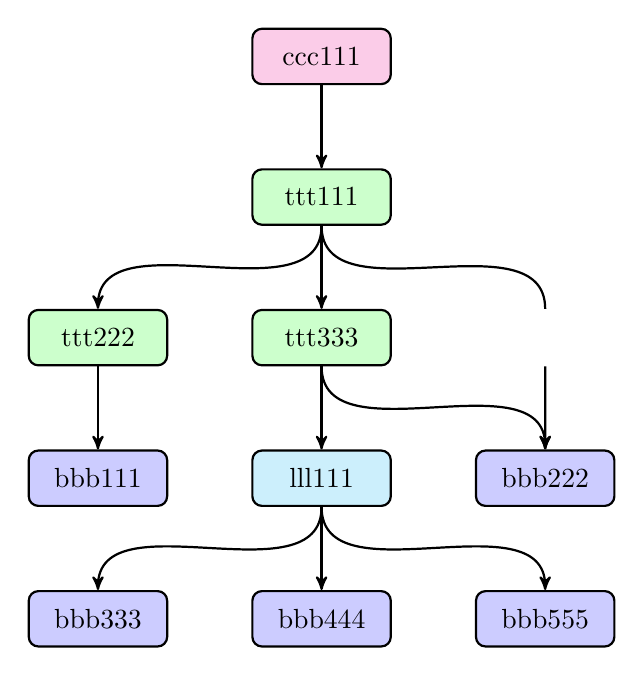
\begin{tikzpicture}[->,>=stealth',auto,thick,
  minimum height=2em,minimum width=5em]

  \tikzstyle{ghost}=[rectangle,rounded corners=.8ex];
  \tikzstyle{block}=[rectangle,draw,fill=blue!20,rounded corners=.8ex];
  \tikzstyle{list}=[rectangle,draw,fill=cyan!20,rounded corners=.8ex];
  \tikzstyle{tree}=[rectangle,draw,fill=green!20,rounded corners=.8ex];
  \tikzstyle{commit}=[rectangle,draw,fill=magenta!20,rounded corners=.8ex];
  \tikzstyle{every path}=[draw]

  \node[commit] (ccc111) {ccc111};
  \node[tree]   (ttt111) [below=3em of ccc111] {ttt111};
  \node[tree]   (ttt222) [below left=3em and 3em of ttt111] {ttt222};
  \node[tree]   (ttt333) [below=3em of ttt111] {ttt333};
  \node[ghost]  (ghost1) [below right=3em and 3em of ttt111] {};
  \node[list]   (lll111) [below=3em of ttt333] {lll111};
  \node[block]  (bbb111) [below=3em of ttt222] {bbb111};
  \node[block]  (bbb222) [below right=3em and 3em of ttt333] {bbb222};
  \node[block]  (bbb333) [below left=3em and 3em of lll111] {bbb333};
  \node[block]  (bbb444) [below=3em of lll111] {bbb444};
  \node[block]  (bbb555) [below right=3em and 3em of lll111] {bbb555};

  \path[every node/.style={font=\sffamily\small}]
    (ccc111) edge[out=-90,in=90] (ttt111)
    (ttt111) edge[out=-90,in=90] (ttt222)
             edge[out=-90,in=90] (ttt333)
             to  [out=-90,in=90]  (ghost1)
             to  [out=-90,in=90] (bbb222)
    (ttt222) edge[out=-90,in=90] (bbb111)
    (ttt333) edge[out=-90,in=90] (lll111)
             edge[out=-90,in=90] (bbb222)
    (lll111) edge[out=-90,in=90] (bbb333)
             edge[out=-90,in=90] (bbb444)
             edge[out=-90,in=90] (bbb555)
  ;

\end{tikzpicture}
\caption{Sample Object Graph} \label{fig:sample-object-graph}

\begin{verbatim}
    # ccc111 contents
    commit 313
    tree ttt111
    author <author public key> <ISO UTC date>
    committer <committer public key> <ISO UTC date>

    # ttt111 contents
    tree 3 250
    tree ttt222 46 ttt222-name
    tree ttt333 166 ttt333-name
    block bbb222 11 bbb222-name

    # ttt222 contents
    tree 1 10
    block bbb111 10 bbb111-name

    # ttt333 contents
    tree 2 104
    list lll111 93 lll111-name
    block bbb222 11 bbb222-eman

    # lll111 contents
    list 3 39
    block bbb333 12
    block bbb444 13
    block bbb555 14

    # bbb111 contents      # block bbb222 contents
    block 1                block 2
    1                      22

    # bbb333 contents      # block bbb444 contents
    block 3                block 4
    333                    4444

    # bbb555 contents
    block 5
    55555
\end{verbatim}
\caption{Sample Objects} \label{fig:sample-objects}
\end{figure}

For example, given the sample objects in Figures \ref{fig:sample-object-graph} and \ref{fig:sample-objects}:

\begin{verbatim}
    # to access tree ttt333:
    ccc111/ttt333-name

    # to access block bbb222:
    ccc111/bbb222-name
    ccc111/ttt333-name/bbb222-eman

    # to access list lll111:
    ccc111/ttt333-name/lll111-name

    # to access block bbb555:
    ccc111/ttt333-name/lll111-name/2
\end{verbatim}

Note that:
\begin{itemize}
  \item[(a)] blocks have no children \\
             \texttt{.../<block>/<child>} is impossible
  \item[(b)] commits implicitly access their trees \\
             \texttt{.../<commit>/name}
             looks up \texttt{"name"} in \texttt{<commit>}'s \texttt{<tree>}
  \item[(c)] \texttt{list} children are accessed by their index \\
             \texttt{.../<list>/4} looks up the fifth block.
\end{itemize}

\paragraph{Path Lookup Performance}

Path-based access traverses the object graph. Retrieving
each object requires potentially looking up its key in the DHT,
connecting to peers, and retrieving its blocks. This is considerable
overhead, particularly when looking up paths with many components.
This is mitigated by:
\begin{itemize}
  \item \textbf{tree caching}: since all objects are hash-addressed, they
        can be cached indefinitely. Additionally, \texttt{trees} tend to be
        small in size so IPFS prioritizes caching them over \texttt{blocks}.
  \item \textbf{flattened trees}: for any given \texttt{tree}, a special
        \texttt{flattened tree} can be constructed to list all objects
        reachable from the \texttt{tree}. Figure \ref{flattened-ttt111} shows
        an example of a flattened tree. While IPFS does not construct flattened
        trees by default, it provides a function for users. For example,
\end{itemize}

\begin{figure}
\begin{verbatim}
  tree 5 250
  tree ttt222 46 ttt222-name
  block bbb111 10 ttt222-name/bbb111-name
  tree ttt333 166 ttt333-name
  list lll111 93 ttt222-name/lll111-name
  block bbb222 11 ttt333-name/bbb222-eman
  block bbb222 11 bbb222-name
\end{verbatim}
\caption{Flattened Tree for \texttt{ttt111}} \label{fig:flattened-ttt111}
\end{figure}


\subsubsection{Publishing Objects}

IPFS is globally distributed. It is designed to allow the files of millions
of users to coexist together. The \textbf{DHT} with content-hash addressing
allows publishing objects in a fair, secure, and entirely distributed way.
Anyone can publish an object by simply adding its key to the DHT, adding
themselves as a peer, and giving other users the object's hash.

Additionally, the IPFS root directory supports special functionality to
allow namespacing and naming objects in a fair, secure, and distributed
manner.
\begin{itemize}
  \item[(a)] All objects are accessible by their hash. Thus, users can
        always reference an object (and its children) using
        \texttt{/<object\_hash>}.

  \item[(b)] \texttt{/<node\_id>} provides a self-certifying filesystem
        for user \texttt{node\_id}. If it exists, the object returned is a
        special \texttt{tree} signed by \texttt{node\_id}'s private key. Thus,
        a user can publish a \texttt{tree} or \texttt{commit} under their
        name, and others can verify it by checking the signature matches.

  \item[(c)] If \texttt{/<domain>} is a valid domain name, IPFS
        looks up key \texttt{gfs} in its \texttt{DNS TXT} record. IPFS
        interprets the value as either an object hash or another IPFS path:
        \begin{verbatim}
  # this DNS TXT record
  fs.benet.ai. TXT "gfs=/aabbccddeeffgg ..."

  # behaves as symlink
  ln -s /aabbccddeeffgg /fs.benet.ai
        \end{verbatim}

\end{itemize}


\subsection{Local Objects}

IPFS clients require some \textit{local storage}, an external system
on which to store and retrieve local raw data for the objects IPFS manages.
The type of storage depends on the node's use case.
In most cases, this is simply a portion of disk space (either managed by
the native filesystem, or directly by the IPFS client). In others, non-
persistent caches for example, this storage is just a portion of RAM.

Ultimately, all blocks available in IPFS are in some node's
\textit{local storage}. And when nodes open files with IPFS, the objects are
downloaded and stored locally, at least temporarily. This provides
fast lookup for some configurable amount of time thereafter.

\subsubsection{Object Pinning}

Nodes who wish to ensure the survival of particular objects can do so by
\texttt{pinning} the objects. This ensures the objects are kept in the node's
\textit{local storage}. Pinning can be done recursively, to pin down all
descendent objects as well. For example, recursively pinning a \texttt{tree}
or \texttt{commit} ensures \textit{all} objects pointed to are stored locally
too. This is particularly useful for nodes wishing to keep all their own files.


%\section{Acknowledgments}


%\bibliographystyle{abbrv}
%\bibliography{gfs}
%\balancecolumns
%\subsection{References}
\end{document}
